\vspace*{\subsecspace}
\section{Policies For Ameliorating Constrained Preemptions}
\label{sec:policies}
Having analyzed the statistical behavior of constrained preemptions and presented our probability model, we now examine how the bathtub shape of the failure rate impacts applications. 
Based on insights drawn from our statistical analysis and the model, we develop various policies for ameliorating the effects of preemptions. 
Prior work in transient computing has established the benefits of such policies for a broad range of applications. 
However, the constrained nature of preemptions introduces new challenges that do not arise in other transient computing environments such as Amazon EC2 spot instances, and thus new approaches are required. 
In this section, we first analyze the impact of constrained preemptions on job running time, and then develop new constrained-preemption aware policies for job scheduling and cost optimization. 

% hl
% hl 

\noindent \textbf{Workload Assumptions.}
Our primary focus is on long-running batch jobs that arise in many scientific computing applications. 
Our scheduling policy assumes that \emph{approximate} job running times are known: which is often the case with ``bags of jobs'', as described in the next section. 
Specifically, we only require knowledge of whether the job running time is above or below a threshold.
% Parallel jobs? Fault model? 0
%Extensions of our models and policies to distributed applications with different failure semantics is part of our future work. 


%, which we present below. 

% For applications running on transient servers, the effects of preemptions can be ameliorated through different policies for fault tolerance and resource management.
% Prior work in transient computing has established the benefits of such policies for a broad range of applications. 
% We now show how our empirical insights and analytical model can be used to develop policies for optimized execution of batch applications on Google Preemptible VMs. 

%We propose to develop optimized preemption mitigating policies that make fundamental use of insights from our models and highlight their practical significance. 

%Our goal is to develop a cost-optimizing execution platform for  batch applications, especially MPI-based scientific computing applications [6] whose large computing requirements and disruption-tolerance make them an ideal application for Preemptible VMs. 
%In particular, the bathtub and time-dependent failures of Preemptible VMs require new policies for these fault-tolerance and resource management problems: 


%\noindent \textbf{High-level System Architecture:} 

%%%%%%%%%%%%%%%%%%%%%%%%%%%%%%%%%%%%%%%%%%%%%%%%%%

\vspace*{\subsecspace}
\subsection{Job Running Time Modeling}

SciSpot uses our bathtub probability model to predict the total running time (i.e., the makespan) of the job. 
% We now look at how temporally constrained preemptions impact the total expected running time of applications by using our failure probability model. 
%
When a preemption occurs during the job's execution, it results in wasted work, assuming there is no checkpointing. 
This increases the job's total expected running time, since it must restart after a preemption.
%
The expected wasted work depends on two factors:
\begin{enumerate} [leftmargin=12pt]
\item The probability of the job being preempted during its execution. 
\item \emph{When} the preemption occurs during the execution. 
\end{enumerate}

We can analyze the wasted work due to a preemption using the failure probability model.
We first compute the expected amount of wasted work \emph{assuming} the job faces a single preemption, which we denote by $E[W_1(T)]$, where $T$ is the original job running time (without preemptions):
\begin{equation}
E[W_1(T)] = \int_0^{T} t~P(t | t \leq T)~dt.
\end{equation}
Here, $P(t|t\leq T) = P(t) / P(t \leq T)$. $P(t\leq T)$ is the probability that there is a preemption within time $T$ and is given by $P(t \leq T) = F(T)$, where $F(T)$ is the CDF (Equation \ref{eq:blend1}). 
$P(t)$ is the probability of a preemption at time $t$, and is given by $P(t) = f(t)$, where $f(t)$ is the preemption rate (Equation~\ref{eq:failrate}).
We can therefore write the above equation as:
% \begin{align}
%   E[W_1(T)] &= \int_0^{T} t~P(t | t \leq T)~dt \nonumber 
%   = \int_0^{T} t~\frac{f(t)}{P(t \leq T)}~dt \\ 
%   &= \int_0^{T} t~\frac{f(t)}{F(T)}~dt 
%     = \frac{1}{F(T)}  \int_0^{T} t~f(t)~dt
%     \label{eq:wasted}
% \end{align}
\begin{equation}
  E[W_1(T)] = \int_0^{T} t~P(t | t \leq T)~dt = \frac{1}{F(T)}  \int_0^{T} t~f(t)~dt.
    \label{eq:wasted}
\end{equation}

We note that the integral is the same as the ``expected lifetime'', given by Equation~\ref{eq:expected-lifetime}.
%
The above expression for the expected waste due to a single preemption can be used by users and application frameworks to estimate the increase in running time due to preemptions. %and other scenarios.
The total running time (also known as makespan) of a job \emph{with} preemptions is given by:
\begin{equation}
  \label{eq:tot-run-time}
  E[T] = P(\text{no failure})~T + P(\text{1 failure})~\left(T + E[W_1(T)]\right),
\end{equation}
where $P(\text{no failure}) = P(t > T) =  1- F(T)$ and $P(\text{1 failure}) = P(t \leq T) = F(T)$.
%The above equation for $E[T]$ thus becomes: 
Expanding out these terms and using Equation \ref{eq:wasted}, we get
%
% \begin{align}
%   \label{eq:tot-run-time-2}
%   E[T] &= (1-F(T))~T + F(T)~(T + E[W_1(T)]) \\ \nonumber
%   &= (1-F(T))~T + F(T)~T + \int_0^{T} t~f(t)~dt \\ \nonumber
%        &= T + \int_0^{T} t~f(t)~dt         
% \end{align}
\begin{align}
  \label{eq:tot-run-time-2}
  E[T] &= \left(1-F\left(T\right)\right)T + F(T)\left(T + E[W_1(T)]\right) \notag \\
  &= T + \int_0^{T} t~f(t)~dt.         
\end{align}
%hl
This expression for the expected running time assumes that the job will be preempted at most once.
An expression which considers multiple ($>1$) job failures easily follows from this base case, but presents relatively low practical value.
% hl

%and most transient computing systems seek to avoid repeated preemptions, and discard the job if multiple preemptions occur or move them to on-demand VMs. 
%hl 

% since they want to avoid pathological behavior of preemptions. 
% This assump, which is a used by transient computing systems to minimize the effect of repeated preemptions. 
% This can be due to multiple reasons: if a job is preempted twice, it may be prudent to move it to an non-preemptible on-demand VM, or delay its execution to a later time when the preemption rate decreases.

\noindent \textbf{Consequences for applications.}
Based on our analysis, both the increase in wasted time ($E[W_1(T)]/T$) and expected running time $(E[T]/T)$ depend on the length of the job for non-memoryless constrained preemptions. 
For memoryless exponential distributions, the expected waste is simply $T/2$, but this assumption is not valid for constrained preemptions, and thus job lengths must be considered when evaluating the suitability of Preemptible VMs. 


Users and transient computing systems can use the expected running time analysis for scheduling and monitoring purposes.
Since the preemption characteristics are dependent on the type of the VM and temporal effects, this analysis also allows principled \emph{selection} of VM types for jobs of a given length. 
% Model-based insight? 
For instance, VMs having a higher initial rate of preemptions are particularly detrimental for short jobs, because the jobs will see high rate of failure and are not long enough to run during the VM's stable period with low  preemption rates. 
We evaluate the expected wasted time and running time for Google Preemptible VMs later in Section~\ref{sec:eval}. 

\vspace*{\subsecspace}
\subsection{Transition-Points based Job Scheduling and VM Reuse Policy}
\label{subsec:sched-policy}

%The time-dependent bathtub preemption rates provide new challenges and opportunities in preemption-mitigation, that do not arise under memoryless preemptions. 
%
Our bathtub probability model also allows us to develop optimized job-scheduling policies for \emph{reducing} job-failures in the bag of jobs execution model. 
%, which we develop in this subsection. 
%
%Many cloud-based applications and services are \emph{long-running}, and typically run a continuous sequence of tasks and jobs on cloud VMs.
%
In the case of deadline-constrained bathtub preemptions, we face a choice: we can either run a new job on an already running VM, or relinquish the VM and run the job on a \emph{new} VM. 
This choice is important in the case of non-uniform failure rates, since the job's failure probability depends on the ``age'' of the VM. 
Because of the bathtub failure distribution, VMs enjoy a long period of low failure rates during the middle of their total lifespan.
Thus, it is beneficial to \emph{reuse} VMs for multiple jobs, and relinquishing VMs after every job completion may not be an optimal choice. 

%Model-based insight? 

However, jobs launched towards the end of VM life face a tradeoff.
While they may start during periods of low failure rate, the 24 hour deadline-imposed sharp increase in preemptions poses a high risk of preemptions, especially for longer jobs.
The alternative is to discard the VM and run the job on a new VM. 
However, since newly launched VMs also have high preemption rates (and thus high job failure probability), the choice of running the job on an existing VM vs. a new VM is not obvious. 

% Expand on this about stable regions etc. 
Our job scheduling policy uses the preemption model to determine the preemption probability of jobs of a given length $T$. 
Assume that the running VM's age (time since launch) is $s$.
%Then, the the probability of failure on the existing VM, $P_{\text{Existing}} = max(1, F(T+s) - F(T))$. 
The intuition is to reuse the VM only if the expected running time is lower, compared to running on a new VM. 
To compute the expected running time of a job of length $T$ starting at vm-age $s$, we  modify our earlier expression for running time (Equation~\ref{eq:tot-run-time-2}) to: % as follows:
\begin{equation}
  \label{eq:tot-run-time-s}
    E[T_s]  = T + \int_{s}^{s+T} t~f(t)~dt
  \end{equation}
The alternative is to discard the VM and launch a new VM, in which case the expected running time is $E[T_0]$. Our job-scheduling policy is simple: 
When a job of running time $T$ attempts to start on a VM of age $s$, if $E[T_s] \leq E[T_0]$, then we run the job on the existing VM.
Otherwise, a new VM is launched.

%\textbf{Practical Relevance:} This policy does not require job running times, only a relative measure if job length is greater or smaller than $E[

% hl

%Depending on the VM's age $s$ and the job's running time $T$, we can compare Equations~\ref{eq:tot-run-time-2} and ~\ref{eq:tot-run-time-s}, and run the job on whichever case yields the lower expected running time. 

\begin{comment}
Our job scheduling policy uses the preemption model to determine the preemption probability of jobs of a given length $T$. 
Assume that the running VM's age (time since launch) is $s$. 
Then, the the probability of failure on the existing VM, $P_{\text{Existing}} = max(1, F(T+s) - F(T))$.  
The alternative is to discard the VM and launch a new VM, in which case, the failure probability is $P_{\text{New}} = F(T)$.
Depending on the VM's age $s$ and the job's running time $T$, we can compare $P_{\text{Existing}}$ and $P_{\text{New}}$, and run the job on whichever case yields the lower failure probability. 
\end{comment}

% Some more intuitive analysis ? 

%Server preemptions lead to \emph{wasted work}, since the progress made by the job is lost (in the absence of any fault-tolerance).
%Minimizing work wasted due to preemptions is a prerequisite to minimizing cost, and 


\noindent \textbf{Transition Points Policy.}
SciSpot builds on the above insight and determines the job-scheduling and VM-reuse decision. 
Based on different job lengths within a bag of jobs and the age of the VM, we minimize the total expected running time of a job.
For any job running time (T), and VM age (s), we compute  $\delta(s,T) = E[T_s] - E[T]$.
If $\delta(s,T) \geq 0$, then a new VM is used, as illustrated in Figure~\ref{fig:transition-example}.
% hl 
%for the VM age $s$, we locate transition point $t*$


Figure~\ref{fig:transition-example} shows that reusing VMs is preferred for shorter job lengths, and the range of jobs for which reusing is good depends on the current age of the VM: younger VMs ($s=1$ hour) can be used for longer job lengths compared to older VMs. 
For a given VM type, we precompute this function for different $(s, T)$ values, and find the transition points where launching a new VM is suitable. 
The precomputed $\delta(s,T)$ can be seen in Figure~\ref{fig:transition-boundary}.
We \emph{analytically} compute the transition point ``frontier'' which is deliniates the re-use vs. new VM portion of the figure. 
Given the VM age $s$, we only need to determine whether the job length is greater or smaller than the transition point. 
This policy has the practical advantage that accurate job running times are not needed---we only require running times relative to the transition point. 
Using this figure, SciSpot, and users in general, can simply lookup the job and VM attributes, and determine the optimal decision. 


%Because the expected job running times are monotonic in $T$, there is a \emph{transition point}
%Our model can also be used to find the transition boundary in the job scheduling policy. The decision to reuse or launch a new VM depends


\begin{figure}[t]
  \subfloat[Difference in expected running times vs. job length $T$ for different VM age $s$. All times are in hours. \label{fig:transition-example}]
  {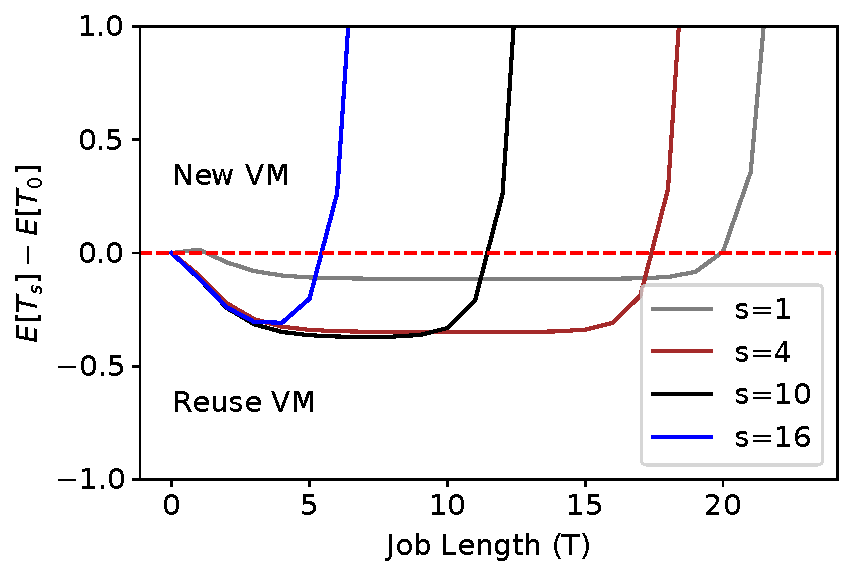
\includegraphics[width=0.26\textwidth]{../graphs/transition-all.pdf}}
  \hfill
  \subfloat[Transition boundary depends on job length and when the job starts on the VM. \label{fig:transition-boundary}]
  {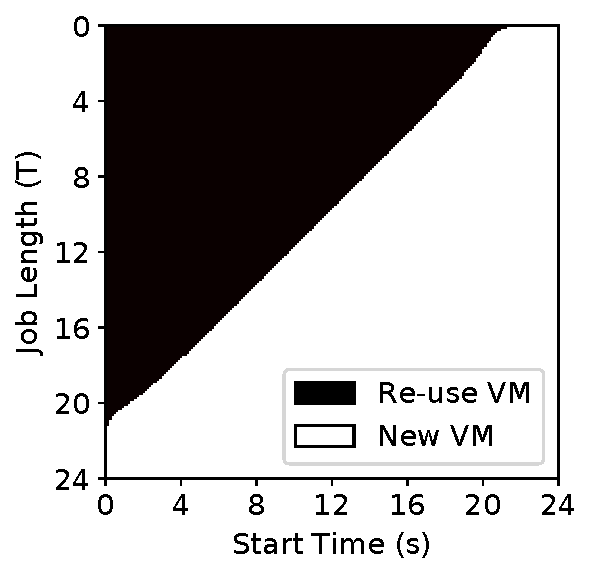
\includegraphics[width=0.2\textwidth]{../graphs/tipping.pdf}}
  \label{fig:transition-all}
  \caption{Reusing vs. running on a new VM.}
\end{figure}

%
\begin{comment}
$d \geq 0 $ implies reusing the VM will yield longer expected time, and thus launching a new VM is preferable.

We can simplify $\delta(s,T) = \int_{s}^{s+T} t~f(t)~dt - \int_{0}^{T} t~f(t)~dt$.

  
  We note that integration by parts yields:
$\int_{0}^{T} t~f(t)~dt = TF(T) - \int_0^T F(t)~dt $.

$\int_{s}^{s+T} t~f(t)~dt = (s+T)F(s+T) - sF(s) - \int_s^{s+T} F(t)~dt $.

%
We can thus obtain:


$\frac{d \delta}{dt} = -1$

$\delta = \int_0^sF(t)~dt - T $

$\frac{d \delta}{d S} = F(s) $

Rate of change of the transition points with respect to start time. 


The model can also be used for 

This technique can also be used to find the job length $T^*$, when the transition occurs between re-using and launching a new VM. 
%
Accurate job lengths are not necessary, and we only need to know whether $T<T^*$, and only a rough estimate of the job lengths is required.
We assume that because most scientific computing workloads involve exploration of some parameter space, they often have homogenenous running times. 
% hl
\end{comment}


\begin{comment}
\vspace*{\subsecspace}
\subsection{Checkpointing Policy}


A common technique for reducing the total expected running time of jobs on transient servers is to use fault-tolerance techniques such as periodic checkpointing \cite{flint}.
%
However, the bathtub nature of constrained preemptions requires new checkpointing policies that do not assume memoryless preemptions. 


Checkpointing application state to stable storage (such as network file systems or centralized cloud storage) reduces the amount of \emph{wasted work} due to preemptions.
However, each checkpoint entails capturing, serializing, and writing application state to a disk, and increases the total running time of the application.
Thus, the frequency of checkpointing can have a significant effect on the total expected running time.

Existing checkpointing systems for handling hardware failures in high performance computing, and for cloud transient servers such as EC2 spot instances, incorporate the classic Young-Daly~\cite{dongarra_fault_nodate, daly2006higher, flint, marathe2014exploiting} periodic checkpointing interval that assumes that failures are exponentially distributed and memoryless.  
That is, the application is checkpointed every $\tau = \sqrt{2 \cdot \delta \cdot \text{MTTF}}$ time units, where $\delta$ is the time overhead of writing a single checkpoint to disk. 


However, checkpointing with a uniform period is sub-optimal in case of time dependent failure rates, and especially for bathtub failure rates. 
A sub-optimal checkpointing rate can lead to increased recomputation and wasted work, or result in excessive checkpointing overhead. 
Intuitively, the checkpointing rate should depend on the failure rate, and our analytical preemption model can be used for designing an optimized checkpointing schedule.

We now present our checkpointing policy that uses the preemption model and provides non-uniform, failure-rate dependent checkpointing.
In a nutshell, our policy allows us to compute the optimal checkpointing schedule for jobs of different lengths and different starting times, employing a dynamic programming approach that minimizes the total expected makespan. 

%%%%%%%%%%%%%%%%%%%%%%%%%%%%%%

\noindent \textbf{Algorithm description:}
Let the uninterrupted running time of the job be $J$.
%In other words, $J$ amount of work needs to be performed.
For ease of exposition, we assume that each job-step takes one unit of time, yielding $J$ job-steps. 
Let the checkpoint cost be $\delta$---i.e, each checkpoint increases the running time by $\delta$. 
We seek to minimize the total expected running time or the \emph{makespan}, which is the sum of $J$, the expected periodic checkpointing cost, and the expected recomputation. 

The makespan $M$ can be recursively defined and computed.
Let $M(J, t)$ denote the makespan where $J$ is remaining length of job to be executed, and $t$ is the time elapsed since the  VM's starting time (i.e., the VM's current age). 
We now need to determine when to take the \emph{next} checkpoint, which we take after $i$ steps. Let $E[M^*]$ denote the minimum expected makespan.
\begin{equation}
  \label{eq:m0}
  E[M^*(J, t)] = \min_{0<i\leq J}{E[M(J, t, i)]}.
\end{equation}
The makespan is affected by whether or not there is a preemption \emph{before} we take the checkpoint: 
\begin{equation}
  \label{eq:m1}
E[M(J, t, i)] = P_{\text{succ}}(t, i+\delta) \cdot E[M_{\text{succ}}] + P_{\text{fail}}(t, i+\delta) \cdot E[M_{\text{fail}}].
\end{equation}
Here $P_{\text{succ}}(t, i+\delta)$ denotes the probability of the job successfully executing without failures until the checkpoint is taken, i.e., from $t$ to $t+i+\delta$. $P_{\text{fail}}(t, i+\delta) = F(t+i+\delta)-F(i+\delta)$ is computed using the CDF, 
and $P_{\text{succ}} = 1 - P_{\text{fail}}$ .


$E[M_{\text{succ}}]$ is the expected makespan if there are no job failures when the job is executing from step $t$ to $t+i+\delta$, and is given by a recursive definition:
\begin{equation}
  \label{eq:msuc}
E[M_{\text{succ}}(J, t, i)] = t+i+\delta + E[M^*(J-i, t+i+\delta)].  
\end{equation}
\noindent The makespan includes the amount of work already done ($t+i$), the checkpointing overhead ($\delta$), and the expected minimum makespan of the rest of the job. 
Similarly, when the job fails before step $i$, then that portion is ``lost work'', and can be denoted by $E[L(t, i+\delta)]$ which is the expected lost work when there is a preemption during the time interval $t$ to $t+i+\delta$.
A preemption before the checkpoint results in no progress, and $J$ steps of the job still remain. 
The expected makespan in the failure case is then given by:
\begin{equation}
  \label{eq:mfail}
 E[M_{\text{fail}}(J, t, i)] = E[L(t, i+\delta)] + E[M^*(J, t+i+\delta)].
\end{equation}



In the case of memoryless preemptions, $E[L(t, i+\delta)]$ is approximated as $\frac{i+\delta}{2}$.
For bathtub preemptions, the lost work is the wasted work that we defined earlier in Equation~\ref{eq:wasted}, but we need to consider the different start and end times, and we get:
\begin{equation}
  \label{eq:exploss}
E[L(t, i+\delta)] = \int_{t}^{t+i+\delta}{x~f(x)~dx}   , 
\end{equation}
where $f(x)$ is the probability density function from Equation~\ref{eq:failrate}.

\noindent \textbf{Computing the optimal checkpoint schedule:}
We can find the minimum makespan $E[M^*(J, t)]$ by using Equations~\ref{eq:m0}--\ref{eq:exploss}. 
Given a job of length $J$, minimizing the total expected makespan involves computing $E[M^*(J, s)]$, where $s$ is the current age of the server. 
Since the makespan is recursively defined, we can do this minimization using dynamic programming, and extract the job-steps at which checkpointing results in a minimum expected makespan. 
%Once all the values of $E[M(J, t, i)]$ are computed, T
The job's checkpointing schedule is determined as follows (assume the job starts at $s=0$ for ease of exposition). 
We first locate the checkpointing interval $i_1$ that minimizes $E[M(J,0,i)]$.  
Then, we recursively find the next checkpointing interval $i_2$ by minimizing  $E[M(J-i_1, i_1,i)]$, and so on, until the $J\leq0$. %Each $E[M(a, b, c)]$ is obtained with a simple lookup in the generated dynamic programming table. 

If a job encounters a failure, it is resumed from the most recent checkpoint, on a new VM.
After every such resume-event, we compute the optimal checkpointing schedule for $E[M^*(J_{\text{Remaining}}, 0)]$, since the job's failure rate is dependent on the VM age when it starts, and the job may be resumed at a later time or on a VM of a different type, etc.
Our algorithm yields non-uniform intervals proportional to failure rate.
For a 5 hour job launched on a new VM (time=0), the checkpointing intervals are $(15, 28, 38, 59, 128)$ minutes.
More checkpointing analysis is presented in Section~\ref{subsec:eval-ckpt}. 

% Explain how 
\end{comment}

%%%%%%%%%%%%%%%%%%%%%%%%%%%%%%%%%%%%%%%%%%%%%%%%%%
\subsection{Cost-aware VM Selection}
\label{subsec:vm-selection}

VM-selection is an important optimization in cloud environments, because VMs have different tradeoffs of cost, performance, and preemption characteristics. 
Application performance is affected by the size of the VM (due to network communication and parallel scaling overheads), and the preemption rates. 
Our policy selects the ``right'' type of  VMs that minimizes the expected job failure probability and cost by using the analytical preemption models. 
%using our model to \emph{compute the expected average lifetime of a VM} enabling us to minimize the impact of preemptions on performance and overall cost.
%Our evaluation indicates that careful VM selection can reduce costs by  up to 30\% compared to 



%%%%%%%%%%%%%%%%%%%%%%%%%%%%%%%%%%%%%%%%%%%%%%%%%%


%\begin{comment} % This is more from the parallelism angle.. 
%We note that this search is different from conventional speedup plots in which the objective is to determine how well an application scales with increasing amount of resources and parallelism. 
%In contrast, we \emph{fix} the total amount of resources allocated to the application's job ($=\mathcal{R}$), and only vary \emph{how} these resources are distributed, which affects communication overhead and hence the performance.
%Weak
%
%Since server selection involves a tradeoff between cost, performance, and preemptions, we develop a model that allows us to optimize the resource allocation and pick the best VM type that minimizes the expected cost of running an application on \sysname. 
%Let $\mathcal{R}$ denote the total amount of computing resources requested for the job. For ease of exposition, let us assume that $\mathcal{R}$ is the total number of CPU cores.
%Furthermore, let $r_i$ denote the ``size'' of the server of type $i$.
%Then, the number of servers of type $i$ required, $n_i = \mathcal{R}/r_i$.
%In what follows, we denote the expectation value of a quantity as $E[\ldots]$.

%\vj{there is some repitition in defining the symbols here which are used before in selection policy; may be this can be moved above. was wondering if we loose clarity by using $T_k$ to denote the running time on configuration $k$ that encodes the pair defined by the combination of server type $i$ - number of servers of type $i$ -- $(i,n_i)$; that is, $k\equiv (i,n_i)$, used as a superindex?}
We assume that the total resource requirement for a job, $\mathcal{R}$, is provided by the user based on prior speedup data, the user's cloud budget, and the deadline for job completion.
Assume that the cloud provider offers $N$ server types, with the price (per unit time) of a server type equal to $c_i$. 
The overall expected cost of running a job is: 
\begin{equation}
  \label{eq:e-cost}
\vspace*{\eqnspace}
  E[C_{( i,n_i )}] = n_i\times c_i \times E[\mathcal{T}_{( i,n_i )}].
\end{equation}
Here, $E[\mathcal{T}_{( i,n_i )}]$ denotes the expected makespan of the job (accounting for preemptions) on $n_i$ servers of type $i$. 
%
This turnaround time depends on whether the job needs to be recomputed because of preemptions, and is given by Equation~\ref{eq:tot-run-time-2}. 
%
\sysname searches over all available and acceptable VM types (modulo any resource constraints on minimum memory/CPUs/GPUs), and picks the VM type which yields the lowest expected cost.
The search process is aided by the bag of jobs abstraction: initial jobs are used for determining the lowest-cost VM, on which the remaining jobs are run. 

%\prat{Highlight tradeoffs here. Larger servers better but more preemption.}



%%%%%%%%%%%%%%%%%%%%%%%%%%%%%%%%%%%%%%%%%%%%%%%%%%

% Using Equations~\ref{eq:turnaround},\ref{eq:recomput}, and \ref{eq:pfail1}, the overall expected cost of running a job on transient cloud servers is obtained as:
% \begin{equation}
%   \label{eq:ecfinal}
%   E[C_{( i,n_i )}] = \frac{1}{2}n_i c_i T_{( i,n_i )}\left(3 - \left(1-\dfrac{T_{( i,n_i )}}{E[L_i]}\right)^{n_i}\right).
% \end{equation}

% Equation \ref{eq:ecfinal} shows that the expected cost $E[C]$ is higher for larger number of servers (high $n_i$), while it is reduced if the expected lifetime of the VM is larger (high $E[L_i]$).



%%% Local Variables:
%%% mode: latex
%%% TeX-master: "paper"
%%% End:
